% file          : doc_tex/basic/Periodic_2_triangulation_2/P2Triang2.tex
% revision      : $Id$
%
% author(s)     : Nico Kruithof <Nico@nghk.nl>

\begin{ccTexOnly}
%\vspace*{-1cm}
\begin{center}
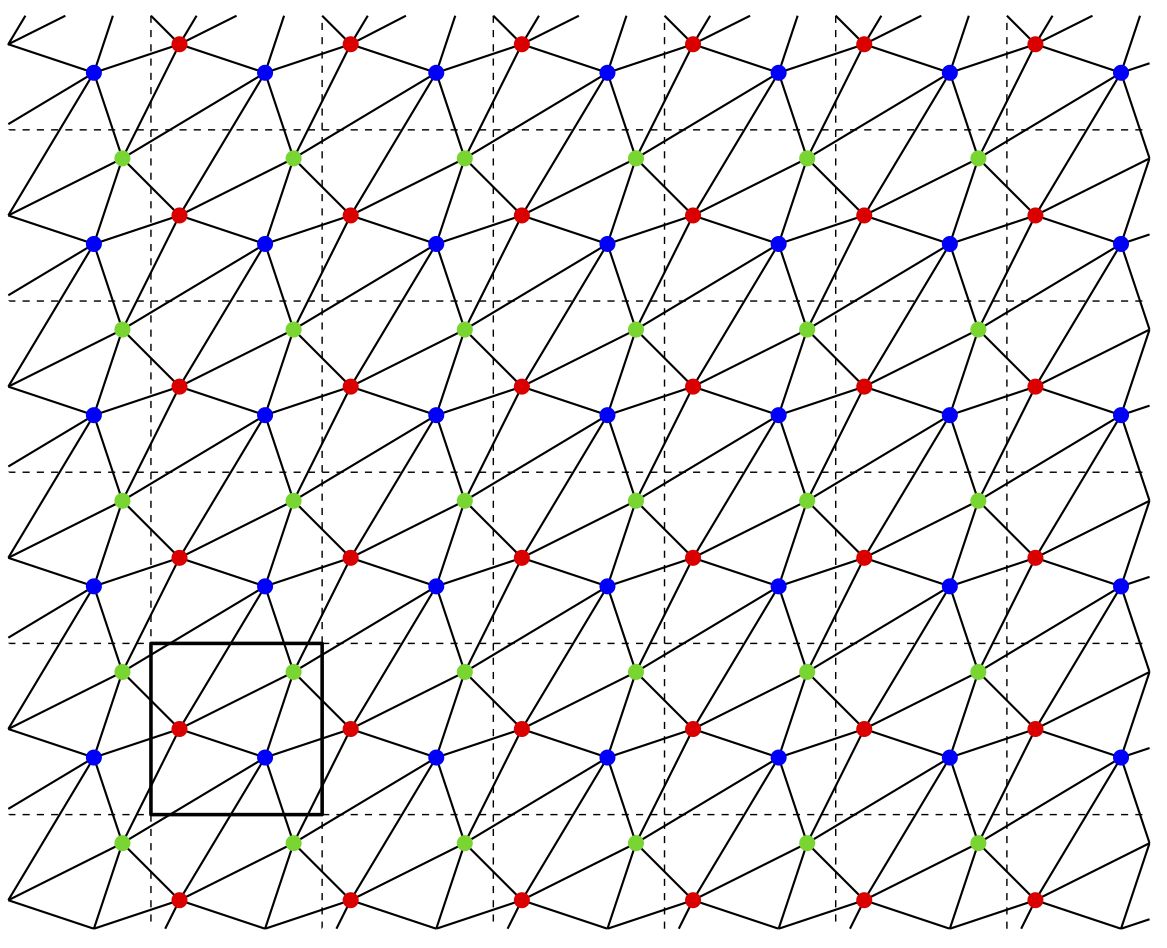
\includegraphics[width=10cm]{Periodic_2_triangulation_2/p2Delaunay2}
\end{center}
\end{ccTexOnly}
\begin{ccHtmlOnly}
<img border=0 src="./p2Delaunay2.png" alt="2D triangulation picture">
\end{ccHtmlOnly}

The periodic 2D-triangulation class of \cgal\ is designed to represent
the triangulation of a set of points in the two-dimensional flat
torus. The triangulation forms a partition of the space it is computed
in. It is a simplicial complex, i.e.\ it contains all incident
$j$-simplices ($j<k$) of any $k$-simplex and two $k$-simplices either
do not intersect or share a common $j$-face, $j<k$. The occurring
simplices of dimension up to two are called \emph{vertex}, \emph{edge}
and \emph{face}, respectively.

\section{The Flat Torus\label{P2Triangulation2-sec-space}}
The 2D Periodic Triangulation package computes triangulations in the
space $\mathbb T_c^2$, which is defined as follows: Let $c\in\mathbb
R\setminus\{0\}$ and $G$ be the group $(c\cdot\mathbb Z^2, +)$, where
$c\cdot\mathbb Z$ denotes the set containing all integer multiples of
$c$. The flat torus is the quotient space: $\mathbb T_c^2:=\mathbb
R^2/G$. The parameter $c$ defines the period.

The elements of $\mathbb T_c^2$ are the equivalence classes of sets of
points in $\mathbb R^2$. We call these points \textit{representatives}
of an element of $\mathbb T_c^2$. The implementation does not work
directly on elements of $\mathbb T_c^2$ but on some representatives in
$\mathbb R^2$. So there need to be distinguished representatives to
work on. Given $\alpha$ and $\beta$, the square
$[\alpha,\alpha+c)\times[\beta,\beta+c)$ contains exactly one
representative of each element in $\mathbb T_c^2$. We call it
\emph{original domain}. From now on, when we talk about
\textit{points}, we generally mean representatives of elements of
$\mathbb T_c^2$ that lie inside the original domain. Note that any
input point is required to be an element of the half-open square
representing the original domain as defined above.

There are simplices containing points inside the original domain but
also points outside it. The points outside the original domain are
periodic copies of points inside the original domain. So, to
specify a simplex we need points together with some additional
information that determines the respective periodic copy of each point. 
The set of representatives of an element of $\mathbb T_c^2$ is a square
point grid. We address each representative by a two-dimensional
integer vector $(o_x,o_y)$, called \emph{offset}. It
represents the number of periods a representative in the original
domain must be translated in $x$- and $y$-direction.
The vector $(0,0)$ corresponds to the representative in the original
domain. To specify a $k$-simplex we need $k+1$ point-offset pairs
(cf.\ Fig.~\ref{P2Triangulation2-fig-offsets}). 

\begin{figure}[htbp]
\begin{ccTexOnly}
\begin{center} 
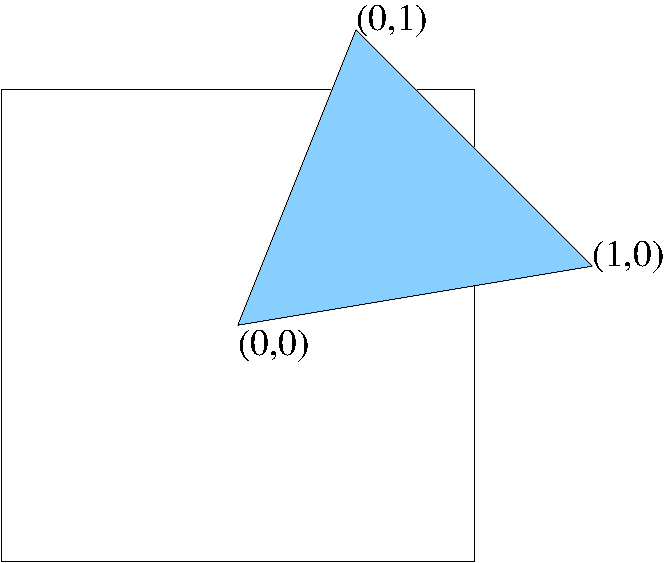
\includegraphics[width=7cm]{Periodic_2_triangulation_2/offsets} 
\end{center}
\end{ccTexOnly}
\begin{ccHtmlOnly}
<CENTER>
<img border=0 src="./offsets.gif" align=middle alt="Offsets in a face.">
</CENTER>
\end{ccHtmlOnly}
\caption{Offsets in a face.
\label{P2Triangulation2-fig-offsets}}
\end{figure} 

\section{Representation\label{P2Triangulation2-sec-intro}}

A triangulation is a collection of vertices and faces that are linked
together through incidence and adjacency relations. Each face gives
access to its three incident vertices, their corresponding offsets, and
to its three adjacent faces. Each vertex gives access to one of its
incident faces.

The three vertices of a face are indexed with 0, 1 and 2 in positive
orientation. The orientation of a simplex in $\mathbb T_c^2$ is
defined as the orientation of the corresponding simplex in $\mathbb
R^2$ given by representatives determined by the respective offsets
(see Figure~\ref{P2Triangulation2-fig-orient}).

\begin{figure}[htbp]
\begin{ccTexOnly}
\begin{center} 
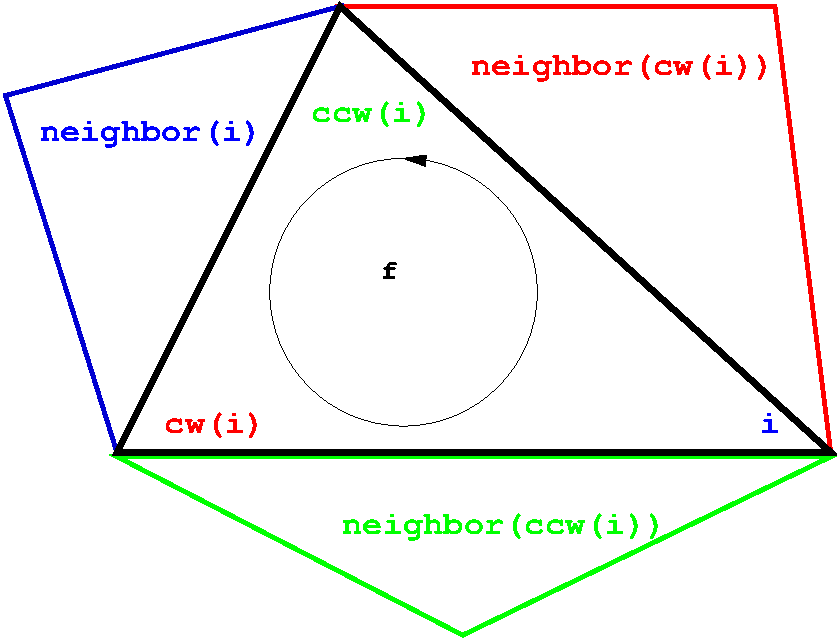
\includegraphics[width=7cm]{Periodic_2_triangulation_2/orient} 
\end{center}
\end{ccTexOnly}
\begin{ccHtmlOnly}
<CENTER>
<img border=0 src="./orient.gif" align=middle alt="Orientation of a face">
</CENTER>
\end{ccHtmlOnly}
\caption{Orientation of a face.
\label{P2Triangulation2-fig-orient}}
\end{figure} 

% TODO(NGHK): Check references to the TDS2
As in the underlying combinatorial triangulation (see
Chapter~\ref{Chapter_2D_Triangulation_Data_Structure}), the neighbors
of a faces are indexed with 0, 1 and 2 in such a way that the neighbor
indexed by $i$ is opposite to the vertex with the same index. Edges
($1$-faces) are not explicitly represented: an edge is given by a face
and an index (the edge \ccc{i} of a face \ccc{f} is the edge of
\ccc{f} that is opposite to the vertex with index \ccc{i}).  See
Figure~\ref{P2Triangulation2-fig-orient}.

Some point sets do not admit a triangulation in $\mathbb T_c^2$. In
this case we use 9 periodic copies of the point set arranged in a
square of edge length $3c$. Any point set constructed in this way has a
triangulation in $\mathbb R^2/G'$ with $G'=(3c\cdot\mathbb Z)^2$
\cite{cgal:ct-c3pt-09}. So we compute the triangulation in this
space, which is a \emph{9-sheeted covering space} of $\mathbb T_c^2$
(see Figure~\ref{P2Triangulation2-fig-covering}).

\begin{figure}[htbp]
\begin{ccTexOnly}
\begin{center} 
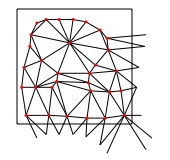
\includegraphics[width=5cm]{Periodic_2_triangulation_2_ref/it_UNIQUE} 
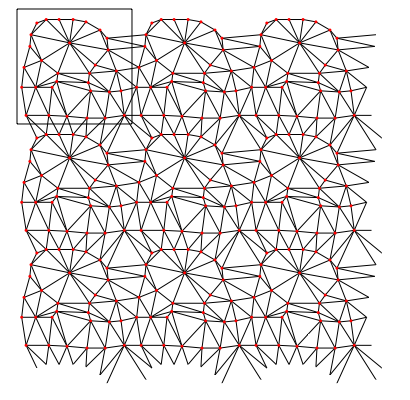
\includegraphics[width=5cm]{Periodic_2_triangulation_2_ref/it_STORED}
\end{center}
\end{ccTexOnly}
\begin{ccHtmlOnly}
<CENTER>
<img border=0 src="../Periodic_2_triangulation_2_ref/it_UNIQUE_small.png"
 align=middle alt="UNIQUE">
<img border=0 src="../Periodic_2_triangulation_2_ref/it_STORED_small.png"
  align=middle alt="STORED">
</CENTER>
\end{ccHtmlOnly}
\caption{The same periodic triangulation in 1-sheeted covering space
  and 9-sheeted covering space.
\label{P2Triangulation2-fig-covering}}
\end{figure} 

The machinery that manages the copies is largely hidden from the
user. However there are some effects that cannot be ignored. For
example if the point set does not permit a triangulation in $\mathbb
T_c^2$ then the combinatorial iterators (\ccc{Face_iterator},
\ccc{Edge_iterator} and \ccc{Vertex_iterator}) return all simplices
that are internally stored, which correspond to 9 periodic copies of
each geometric primitive (Triangle, Segment, and Point). This is
necessary to ensure consistency in the adjacency relations. In case it
is desired to have only one periodic copy of each primitive, we
provide \emph{geometric} iterators. They return geometric primitives
of the triangulation without relations between them. Another effect is
that when the algorithm switches from 9-sheeted covering to 1-sheeted
covering the \ccc{Vertex_handle}s and \ccc{Face_handle}s referencing
deleted items becomes invalid.

In the data structure each vertex stores the input point it
corresponds to. If we are computing in 9-sheeted covering 
space, each vertex stores the representative \emph{inside} the
original domain it corresponds to. So, the 9 vertices corresponding
to the same element of $\mathbb T_c^2$ all store the same
representative in $\mathbb R^2$, and not different periodic copies.

\paragraph{Validity}
A periodic triangulation is said to be \ccc{locally valid} iff

% TODO(NGHK): Check references to the TDS2
{\bf (a)-(b)} Its underlying combinatorial graph, the triangulation
data structure, is \ccc{locally valid}
(see Chapter~\ref{Chapter_2D_Triangulation_Data_Structure})\\
{\bf (c)} Any cell has its vertices ordered according to positive
orientation. See Figure~\ref{P2Triangulation2-fig-orient}.

\section{Delaunay Triangulation} 
The class \ccc{Periodic_2_Delaunay_triangulation_2} implements Delaunay
triangulations of point sets in $\mathbb T_c^2$.

Delaunay triangulations have the \textit{empty circle property},
that is, the circumscribing circle of each face does not contain any
other vertex of the triangulation in its interior. These
triangulations are uniquely defined except in degenerate cases where
four points are co-circular.  Note however that the \cgal\
implementation computes a unique triangulation even in these cases
\cite{cgal:dt-pvr3d-03}.

This implementation is fully dynamic: it supports both insertions of
points and vertex removal (NGHK: TODO, removal of points is not
implemented yet).

\section{Triangulation Hierarchy}
The class \ccc{Periodic_2_triangulation_hierarchy_2} is the adaptation
of the hierarchical structure described in
Chapter~\ref{Chapter_2D_Triangulations},
Section~\ref{Section_2D_Triangulations_Hierarchy} to the periodic
case. (NGHK: TODO, hierarchy is not implemented yet)

The class \ccc{Triangulation_hierarchy_2<Tr>} inherits from the
triangulation type passed as template parameter \ccc{Tr}. 
The \ccc{insert}, \ccc{move}, and \ccc{remove} member functions
are  overwritten to update the data structure at each operation.
The locate queries are also overwritten to take advantage of the data
structure for a fast processing.

\section{Software Design\label{P2Triangulation2-sec-design}}
We have chosen the prefix ``Periodic\_2'' to emphasize that the
triangulation is periodic in all two directions of space. There are
also ``cylindrical'' periodicities where the triangulation is periodic
only in one direction of the space.

The two main classes \ccc{Periodic_2_Delaunay_triangulation_2} and
\ccc{Periodic_2_triangulation_2} provide high-level geometric
functionality and are responsible for the geometric validity.
\ccc{Periodic_2_Delaunay_triangulation_2} contains all the
functionality that is special to Delaunay triangulations, such as
point insertion and vertex removal, the side-of-circle test, finding
the conflicting region of a given point (NGHK: check), dual functions etc.
\ccc{Periodic_2_triangulation_2} contains all the functionality
that is common to triangulations in general, such as location of a
point in the triangulation \cite{cgal:dpt-wt-02}, access functions,
geometric queries like the orientation test etc.

They are built as layers on top of a triangulation data structure,
which stores their combinatorial structure. This separation between
the geometry and the combinatorics is reflected in the software design
by the fact that the triangulation classes take two template
parameters: 
\begin{itemize}
%
\item {} the \textbf{geometric traits} class, which provides the type
  of points to use as well as the elementary operations on them
  (predicates and constructions). Furthermore it contains the offset
  type.  The concept for this parameter is described in more detail in
  Section~\ref{P2Triangulation2-sec-Traits}. The concepts that should
  be refined are \ccc{Periodic_2TriangulationTraits_2} (for
  \ccc{Periodic_2_triangulation_2}) and
  \ccc{Periodic_2DelaunayTriangulationTraits_2} (for
  \ccc{Periodic_2_Delaunay_triangulation_2}) in the reference
  manual\lcTex{ on~\ccRefPage{Periodic_2TriangulationTraits_2}} and
  \lcTex{\ccRefPage{Periodic_2DelaunayTriangulationTraits_2}}.

\item {} the \textbf{triangulation data structure} class, which stores
  the combinatorial structure, described in
  Section~\ref{P2Triangulation2-sec-tds} and in more detail in
  Chapter~\ref{Chapter_2D_Triangulation_Data_Structure}. The
  triangulation data structure needs models of the concepts
  \ccc{Periodic_2TriangulationDSFaceBase_2} and
  \ccc{Periodic_2TriangulationDSVertexBase_2} as template parameters.
\end{itemize}

\subsection{The Geometric Traits Parameter\label{P2Triangulation2-sec-Traits}}
The first template parameter of the periodic triangulation class
\ccc{Periodic_2_triangulation_2<Traits, Tds>} is the geometric traits
class, described by the concept \ccc{Periodic_2TriangulationTraits_2}.
Similar, the first template parameter of the Delaunay triangulation
class \ccc{Periodic_2_Delaunay_triangulation_2<Traits,Tds>} is the
geometric traits class, described by the concept
\ccc{Periodic_2DelaunayTriangulationTraits_2}.  These concepts are
different from the \ccc{TriangulationTraits\_2} and
\ccc{DelaunayTriangulationTraits\_2} (see
chapter~\ref{Triangulation2-sec-Traits}) in that they also implement
all objects, predicates and constructions with using offsets.

The class
\ccc{Periodic_2_Delaunay_triangulation_traits_2<Traits,Periodic_2Offset_2>}
provides the required functionality. It expects two template
parameters: A model of the concept \ccc{DelaunayTriangulationTraits_2}
and a model of the concept \ccc{Periodic_2Offset_2}. Since the concept
\ccc{TriangulationTraits_2} refines the concept
\ccc{DelaunayTriangulationTraits_2}, the class
\ccc{Periodic_2_Delaunay_triangulation_traits_2<Traits,Periodic_2Offset_2>}
is also a model for the concept \ccc{TriangulationTraits_2}.

The kernels \ccc{Cartesian}, \ccc{Homogeneous},
\ccc{Simple_cartesian}, \ccc{Simple_homogeneous} and
\ccc{Filtered_kernel} can all be used as models for
\ccc{Traits}. \ccc{Periodic_2_triangulation_traits_2} provides exact
predicates and exact constructions if \ccc{Traits} does. It provides
exact predicates but not exact constructions if
\ccc{Filtered_kernel<CK>} with \ccc{CK} an inexact kernel is used as
its first template parameter. Using
\ccc{Exact_predicates_inexact_constructions_kernel}\lcTex{
  (\ccRefPage{Exact_predicates_inexact_constructions_kernel})} as
\ccc{Traits} provides fast and exact predicates and not exact
constructions, using
\ccc{Exact_predicates_exact_constructions_kernel}\lcTex{
  (\ccRefPage{Exact_predicates_exact_constructions_kernel})} provides
fast and exact predicates and exact constructions. The latter is
recommended if the dual constructions and constructions of points,
segments, triangles, and tetrahedra are used.

The second parameter \ccc{Periodic_2Offset_2} defaults to
\ccc{Periodic_2_offset_2}.

\subsection{The Triangulation Data Structure Parameter\label{P2Triangulation2-sec-tds}}

The second template parameter of the main classes
\ccc{Periodic_2_triangulation_2} and
\ccc{Periodic_2_Delaunay_triangulation_2} is a
triangulation data structure class.  This class can be seen as a container for
the faces and vertices maintaining incidence and adjacency relations (see
Chapter~\ref{Chapter_2D_Triangulation_Data_Structure}).  A model of this triangulation data structure is
\ccc{Triangulation_data_structure_2}, and it is described by the
\ccc{TriangulationDataStructure_2} concept.  This model is itself
parameterized by a vertex base class and a face base class, which gives the
possibility to customize the vertices and cells used by the triangulation data
structure, and hence by the geometric triangulation using it.
To represent periodic triangulations the cell base and vertex base
classes need to meet the concepts
\ccc{Periodic_2TriangulationDSFaceBase_2} and
\ccc{Periodic_2TriangulationDSVertexBase_2}.

A default value for the triangulation data structure parameter is provided in
all the triangulation classes, so it does not need to be specified by
the user unless he wants to use a different triangulation data
structure or a different vertex or cell base class.

\subsection{Flexibility of the Design}
\ccc{Periodic_2_triangulation_2} uses the
\ccc{TriangulationDataStructure_2} in essentially the same way as
\ccc{Triangulation_2}. That is why the flexibility described in
\ref{Section_2D_Triangulations_Software_Design} is applicable in exactly the same
way. Also the classes \ccc{Triangulation_vertex_base_with_info_2} and
\ccc{Triangulation_face_base_with_info_2} can be reused directly, see
also Example \ref{P2Triangulation2-sec-examples-color}.

\section{Examples\label{P2Triangulation2-sec-examples}}
\subsection{Basic Example}
This example shows the incremental construction of a periodic 2D
Delaunay triangulation, the location of a point and how to perform
elementary operations on indices in a face. It uses the default
parameter of the \ccc{Periodic_2_Delaunay_triangulation_2} class for
the triangulation data structure.

\ccIncludeExampleCode{Periodic_2_triangulation_2/simple_example.cpp}

\subsection{Changing the Vertex Base}
The following two examples show how the user can plug his own vertex
base in a triangulation. Changing the face base is similar.

\subsubsection{Adding a Color\label{P2Triangulation2-sec-examples-color}}
If the user does not need to add a type in a vertex that depends on
the \ccc{TriangulationDataStructure_2} (e.g. a \ccc{Vertex_handle} or
\ccc{Face_handle}), he can use the
\ccc{Triangulation_vertex_base_with_info_2} class to add his own
information easily in the vertices.  The example below shows how to
add a \ccc{CGAL::Color} this way.

\ccIncludeExampleCode{Periodic_2_triangulation_2/colored_vertices.cpp}

\subsubsection{Adding Handles}
If the user needs to add a type in a vertex that depends on the
\ccc{TriangulationDataStructure_2} (e.g. a \ccc{Vertex_handle} or
\ccc{Face_handle}), he has to derive his own vertex base class, as the
following example shows.

\ccIncludeExampleCode{Periodic_2_triangulation_2/periodic_adding_handles.cpp}

\subsection{9-sheeted Covering}
The user can check at any time whether a triangulation would be a
simplicial complex in $\mathbb T_c^2$ and force a conversion if
so. However this should be done very carefully in order to be sure
that the internal structure always remains a simplicial complex and
thus a triangulation.

In this example we construct a triangulation that can be converted to
the 1-sheeted covering. However, we can insert new points such that the
point set does not have a Delaunay triangulation in the 1-sheeted
covering anymore, so the triangulation is not \emph{extensible}.

\ccIncludeExampleCode{Periodic_2_triangulation_2/covering.cpp}


\subsection{Large Point Set}

For large point sets there are two optimizations available. Firstly,
there is spatial sorting that sorts the input points according to a
Hilbert curve, see chapter~\ref{sec:spatial_sorting}\lcTex{ on
\ccRefPage{sec:spatial_sorting}}.
The second one inserts 12 appropriately chosen dummy points to avoid
the use of a 9-sheeted covering in the beginning. The 12 dummy
points are deleted in the end. If the point set turns out to not have
a Delaunay triangulation in 1-sheeted covering, the triangulation is
converted to 9-sheeted covering during the removal of the 12 dummy
points. This might take even longer than computing the triangulation
without using this optimization. In general, uniformly distributed
random point sets of more than 1000 points have a Delaunay
triangulation in 1-sheeted covering.

It is recommended to run this example only when compiled in release
mode because of the relatively large number of points. 

\ccIncludeExampleCode{Periodic_2_triangulation_2/large_point_set.cpp}

\subsection{Geometric Access}

There might be applications that need the geometric primitives of a
triangulation as an input but do not require a simplicial complex. For
these cases we provide the geometric iterators that return only the
geometric primitives fulfilling some properties. In the following
example we use the \ccc{Periodic_triangle_iterator} with the option
\ccc{UNIQUE_COVER_DOMAIN}. This means that only those triangles are
returned that have a non-empty intersection with the original domain
of the 1-sheeted covering space, see
Figure~\ref{P2Triangulation2-fig-geom_iterators}\lcTex{
  \ccRef{P2Triangulation2-fig-geom_iterators}}.
The \ccc{Periodic_triangle} is actually a two-dimensional array of
point-offset pairs. We check for all three entries of the periodic
triangle whether the offset  is (0,0,0) using the
method \ccc{is_null}. If so, we convert the periodic triangle to a
\ccc{PK::Triangle_2}, which requires \emph{exact constructions}.

\ccIncludeExampleCode{Periodic_2_triangulation_2/geometric_access.cpp}

%%%%%%%%%%%%%%%%%%%%%%%%%%%%%%%%
\section{Design and Implementation History}
The periodic 2D-triangulation is based on the 2D triangulation package
developed by Mariette Yvinec and the periodic 3D-triangulation package
developed by Manuel Caroli and Monique Teillaud. The periodic
3D-triangulation package is described in Manuel's PhD thesis
\cite{cgal:c-tpsos-10}.

Triangulating Point Sets in Orbit Spaces In 2009, Nico Kruithof
started implementation of the \ccc{Periodic_2_triangulation_2}
package.

\section{Performance}
The performance of the 2D periodic Delaunay triangulation is compared
to the Euclidean 2D Delaunay triangulation.

NGHK: TODO: Performance benchmark
